\chapter{図表}


\section{浮動体の配置制御\texorpdfstring{\zdash}{---}\Y{afterpage}}
\zindind{浮動体}{の配置}%
\latexno{における浮動体}%

\LaTeX の\Z{浮動体} (\Z{float}) の配置に関しては色々と不満をお持ちの方がいらっしゃ
るようです.%[たくさん...]
例えば,標準的には
\begin{inputex}
\begin{figure}[htbp]
 \begin{center}
    \includegraphics{filename}
    \caption{caption\label{fig:label}}
 \end{center}
\end{figure}
\end{inputex}
としておけば、私は別にどうってことないです。大抵は浮動体に関わるパラメー
タを再定義することにより解決します。\ppl{奥村晴彦}の \Y{jsclasses} では
すでに再定義されているので使いやすいはずです。浮動体に関わるパラメータに
は次のようなものがあります.
\begin{description}
\item[\K{topnumber}\pp{カウンタ}] 
ページ上部に配置することが出来る浮動体の数.
\item[\K{bottomnumber}\pp{カウンタ}]
ページ下部に配置することが出来る浮動体の数.
\item[\K{totalnumber}\pp{カウンタ}]
あるページに配置することが出来る浮動体の総数.
\item[\C{topfraction}\pp{0--1 の実数}]
浮動体がページ上部を占有できる割合.
\item[\C{bottomfraction}\pp{0--1 の実数}]
浮動体がページ下部を占有できる割合.
\item[\C{textfraction}\pp{0--1 の実数}]
文章がページを占有すべき割合.
\item[\C{floatpagefraction}\pp{0--1 の実数}]
浮動体しか含まれないページにおける浮動体の割合.
\item[\K{dbltopnumber}\pp{カウンタ}]
2 段組みにおける \K{topnumber}.
\item[\C{dlbtopfraction}\pp{0--1 の実数}]
2 段組みにおける \C{topfraction}.
\item[\C{dlbfloatpagefraction}\pp{0--1 の実数}]
2 段組みにおける \C{floatpagefraction}.
\item[\C{floatsep}\pp{スキップ}]
ページの上部か下部に出力された浮動体同士の空き.
\item[\C{textfloatsep}\pp{スキップ}]
ページ上部か下部に出力された浮動体と本文の空き.
\item[\C{intextsep}\pp{スキップ}]
ページの中部に出力された浮動体と本文の空き.
\item[\C{dlbfloatsep}\pp{スキップ}]
2 段組みにおける \C{floatsep}.
\item[\C{dlbtextfloatsep}\pp{スキップ}]
2 段組みにおける \C{textfloatsep}.
\end{description}
上記のパラメータの設定方法に関しては別の解説書を参照するなり,クラスファ
イルなどを覗いてみてください.これらを再定義してもだめならば邪道ですが,
フロートさせずに
\begin{inputex}
\makeatletter
\newenvironment{myFigure}{%
   \begin{center}\def\@captype{figure}}{\end{center}}
\makeatother
\begin{myFigure}
   \includegraphics{filename}
    \caption{caption}
\end{myFigure} 
\end{inputex}

とすることにより、浮動体として扱わなくなります (そのかわり、ページの空き
が調整されないなどの副作用もあります) 。既存のマクロパッケージ \Y{here} を使
うことも考えられますが、もっと確実に図を配置したいものです。そこで
\ppl{David Carlisle}の \Y{afterpage} を使います。
\begin{inputex}
\usepackage{afterpage,here}
\afterpage{\clearpage\begin{figure}[H] ... \end{figure}} 
\end{inputex}
とすることによりあらかじめ \C{clearpage} して \Y{here} パッケージを使い、
無理やりそこに配置を試みます。これ以外にも例えば、次ページの先頭になんら
かの要素を配置したい場合は
\begin{inputex}
\afterpage{\clearpage ...}
\end{inputex}
とすることができます。%[こんどやってみます]


\begin{Exe}
次のようにして浮動体に関わる現在のパラメータの値を確認してください.
\begin{inputex}
\newcommand*\checkcnt[1]{\texttt{#1} $=$ 
   \expandafter\the\csname c@#1\endcsname} 
\checkcnt{topnumber}\par
\checkcnt{bottomnumber}\par
\checkcnt{totalnumber}\par
\newcommand*\checkcmd[1]{\texttt{\string#1} $=$ #1}
\checkcmd{\topfraction}\par
\checkcmd{\bottomfraction}\par
\checkcmd{\textfraction}\par
\checkcmd{\floatpagefraction}
\end{inputex}
もしもそのパラメータで満足の行く結果にならなければ,
\begin{inputex}
\renewcommand\topfraction{0.85}
\addtocounter{topnumber}{2}
\end{inputex}
などとして,再定義するなり再設定してみてください.
また,そうした結果,組版結果にどのような違いがあるか考えて
みてください.
\end{Exe}

\section{書籍スタイルの表罫線\texorpdfstring{\zdash}{---}\Y{booktabs}}

どうも日本人は\Z{表組み}で\Z{縦罫線}や\Z{斜線}を使う傾向に
あるようです。典型的な日本人が組んだものは下記のようになります。
なんともけばけばしい感じです。
\begin{InOut}
\begin{tabular}{|l||l|l|}
 \hline
 名称   & 型番  & 個数 \\
 \hline \hline
 たわし & TWS01 & 1000 \\
 \hline
 石鹸   & SP01  & 5000 \\
 \hline
\end{tabular}
\end{InOut}
実際の本作りや欧文での表組みでは上記のような組み方は避けた方が無難です。
\Z{認知心理学}的にもやさしく、記述も簡単な次のような組み方をお薦めします。
\begin{InOut}
\begin{tabular}{lll}
 \hline
 名称   & 型番  & 個数 \\
 \hline
 たわし & TWS01 & 1000 \\
 石鹸   & SP01  & 5000 \\
 \hline
\end{tabular}
\end{InOut}
ただ、もう少し本格的にやろうと思えば、\ppl{Simon Fear}による
\Y{booktabs} を使うと良いでしょう。
\begin{Syntax}
\C{toprule} \pp{表の最上部に引く罫線}\\
\C{midrule} \pp{表の中間に引く罫線}\\
\C{bottomrule} \pp{表の最下部に引く罫線}
\end{Syntax}
\C{toprule} と \C{midrule}、そして \C{bottomrule} の三つを
必ず使うようにします。
\begin{InOut}
\begin{tabular}{lll}
\toprule
品名 & 番号 & 個数 \\
\midrule
たわし & 02A & 3 \\
雑巾   & 55B & 2 \\
傘     & X2B & 5 \\
\bottomrule
\end{tabular}
\end{InOut}

表の中に半端の罫線を引く場合は \C{cmidrule} 命令を使います。
\begin{Syntax}
\C{cmidrule}\pa{罫線を引く範囲}
\end{Syntax}
\C{cmidrule} は \C{multicolumn} などにより列を連結した場合等に
使うことが出来ると思います。
\begin{InOut}
\begin{tabular}{lll}
 \toprule
 \multicolumn{2}{c}{項目} & \\
 \cmidrule{1-2}
 品名 & 型番 & 個数\\
 \midrule
 たわし & 02A & 3 \\
 雑巾   & 55B & 2 \\
 傘     & X2B & 5 \\
 \bottomrule
\end{tabular}
\end{InOut}


\section{小数点揃え\texorpdfstring{\zdash}{---}\Y{dcolumn}}
\E{tabular} 環境などで表を作っていると、\Z{小数点}などで列を\Z{整列}させ
たいときがあります。この場合、手動で次のようにもできます。
\begin{InOut}
 \begin{center}
  \begin{tabular}{|l|r@{.}l|}
   $\sqrt{157}$   & 12 & 53 \\
   $\pi$ & 3 & 141592 \\
  \end{tabular}
 \end{center}
\end{InOut}
しかし、ここは自動的に小数点でそろえて欲しいものです。
小数点などをそろえる一つの方法として \pp{David Carlisle} の \Y{dcolumn}
を使う方法があります。
\begin{Syntax}
\C{newcolumntype}\pa{区切り記号}\pa{入出力に関する設定} \pp{設定のため}\\
\texttt{D}\pa{\TeX での区切り}\pa{DVI での出力形式}\pa{小数部の桁数} \pp{列指定子}
\end{Syntax}
という定義することにより、小数点 `.' に限らず、なんらかの区切りで
列を整列できます。
\begin{InOut}
 \usepackage{dcolumn}
 \begin{center}
  \newcolumntype{.}{D{.}{.}{6}}
  \begin{tabular}{|l|.|}
   $\sqrt{157}$ & 12.53    \\
   $\pi$        & 3.141592 \\
  \end{tabular}
 \end{center}
\end{InOut}
\E{tabular} 環境などで直接\Z{列指定子} `D' を使うことも出来ます。
上記の場合はあらかじめ\Z{ピリオド} `.' を列の整列用の指定子として
登録しています。

\section{ページを跨ぐ表\texorpdfstring{\zdash}{---}\Y{longtable}}
%*** The longtable package by David Carlisle [#x824dcd6]
まぁ、どう頑張ってもページを跨いじゃうような表をたまに作っちゃうわけですが、
このような場合は \ppl{David Carlisle}の \Y{longtable} パッケージでも使
いましょう。 \Y{longtable} パッケージを読み込むことにより \E{longtable}
環境が使えるようになります。

ただし、 \E{table} 環境中にはいれません。また表の幅をそろえるためには、
\Y{longtable}パッケージの警告が出なくなるまで複数回のタイプセットが必要
になります。

ページが複数ページに跨いでしまったときに、各ページの下部・上部に表示させたい
要素が指定できます。
\begin{Syntax}
\va{要素} \C{endfirsthead}\pp{表の最初のページの上部にだけ表示する行の要素}\\
\va{要素} \C{endhead}\pp{行がページを跨ぐとき、各ページの上部に表示する行の要素}\\
\va{要素} \C{endfoot}\pp{行がページを跨ぐとき、各ページの下部に表示する行の要素}\\
\va{要素} \C{endlastfoot}\pp{表の最後のページの下部だけに表示する行の要素}
\end{Syntax}
具体例をみた方が分かりやすいでしょう。次のような入力があると
すると出力は \figref{fig:longtable} となります。
\begin{inputex}
\documentclass[a4j,11pt,papersize]{jsarticle}
\usepackage{longtable}
\newcommand\hoge[1][0]{%
  醤油 #1-0 & 32892378923894832894 & 1000 \\
  醤油 #1-1 & 32892378923894832894 & 1000 \\
  醤油 #1-2 & 32892378923894832894 & 1000 \\
  醤油 #1-3 & 32892378923894832894 & 1000 \\
  醤油 #1-4 & 32892378923894832894 & 1000 \\
  醤油 #1-5 & 32892378923894832894 & 1000 \\
  醤油 #1-6 & 32892378923894832894 & 1000 \\
  醤油 #1-7 & 32892378923894832894 & 1000 \\
  醤油 #1-8 & 32892378923894832894 & 1000 \\
  醤油 #1-9 & 32892378923894832894 & 1000 \\
}
\begin{document}
% 表の幅を取得するために \jobname.aux に longtable パッケージは
% 情報を書き出し、2 回目以上のタイプセットで幅をそろえる。
\newcommand\mytablehead{\hline 商品 & 番号 & 個数 \\}
\begin{longtable}{|l|l|l|}
\caption{長いながーい表\label{tab:longtable}}
% 表の最初のページの上部にだけ表示する行の要素
\endfirsthead
\hline
\multicolumn{3}{|c|}{前ページの表の続きです。}\\
\mytablehead
\hline
% 行がページを跨ぐとき、各ページの上部に表示する行の要素
\endhead
\hline
\multicolumn{3}{|c|}{この表の続きが次ページにあります。}\\
\hline
% 行がページを跨ぐとき、各ページの下部に表示する行の要素
\endfoot
\multicolumn{3}{|c|}{これでこの表は終わりです。}\\
\hline
% 表の最後のページの下部だけに表示する行の要素
\endlastfoot
% 実際の表の始まり
\mytablehead
\hline
\hoge[1] \hoge[2] \hoge[3] \hoge[4] \hoge[5]
\hoge[6] \hoge[7] \hoge[8] \hoge[9] \hoge[10]
\hoge[11] \hoge[12] \hoge[13]
\hline
\end{longtable}
\end{document}
\end{inputex}

\begin{figure}[htbp]
   \IOmargin
   \makebox[0pt][l]{%
      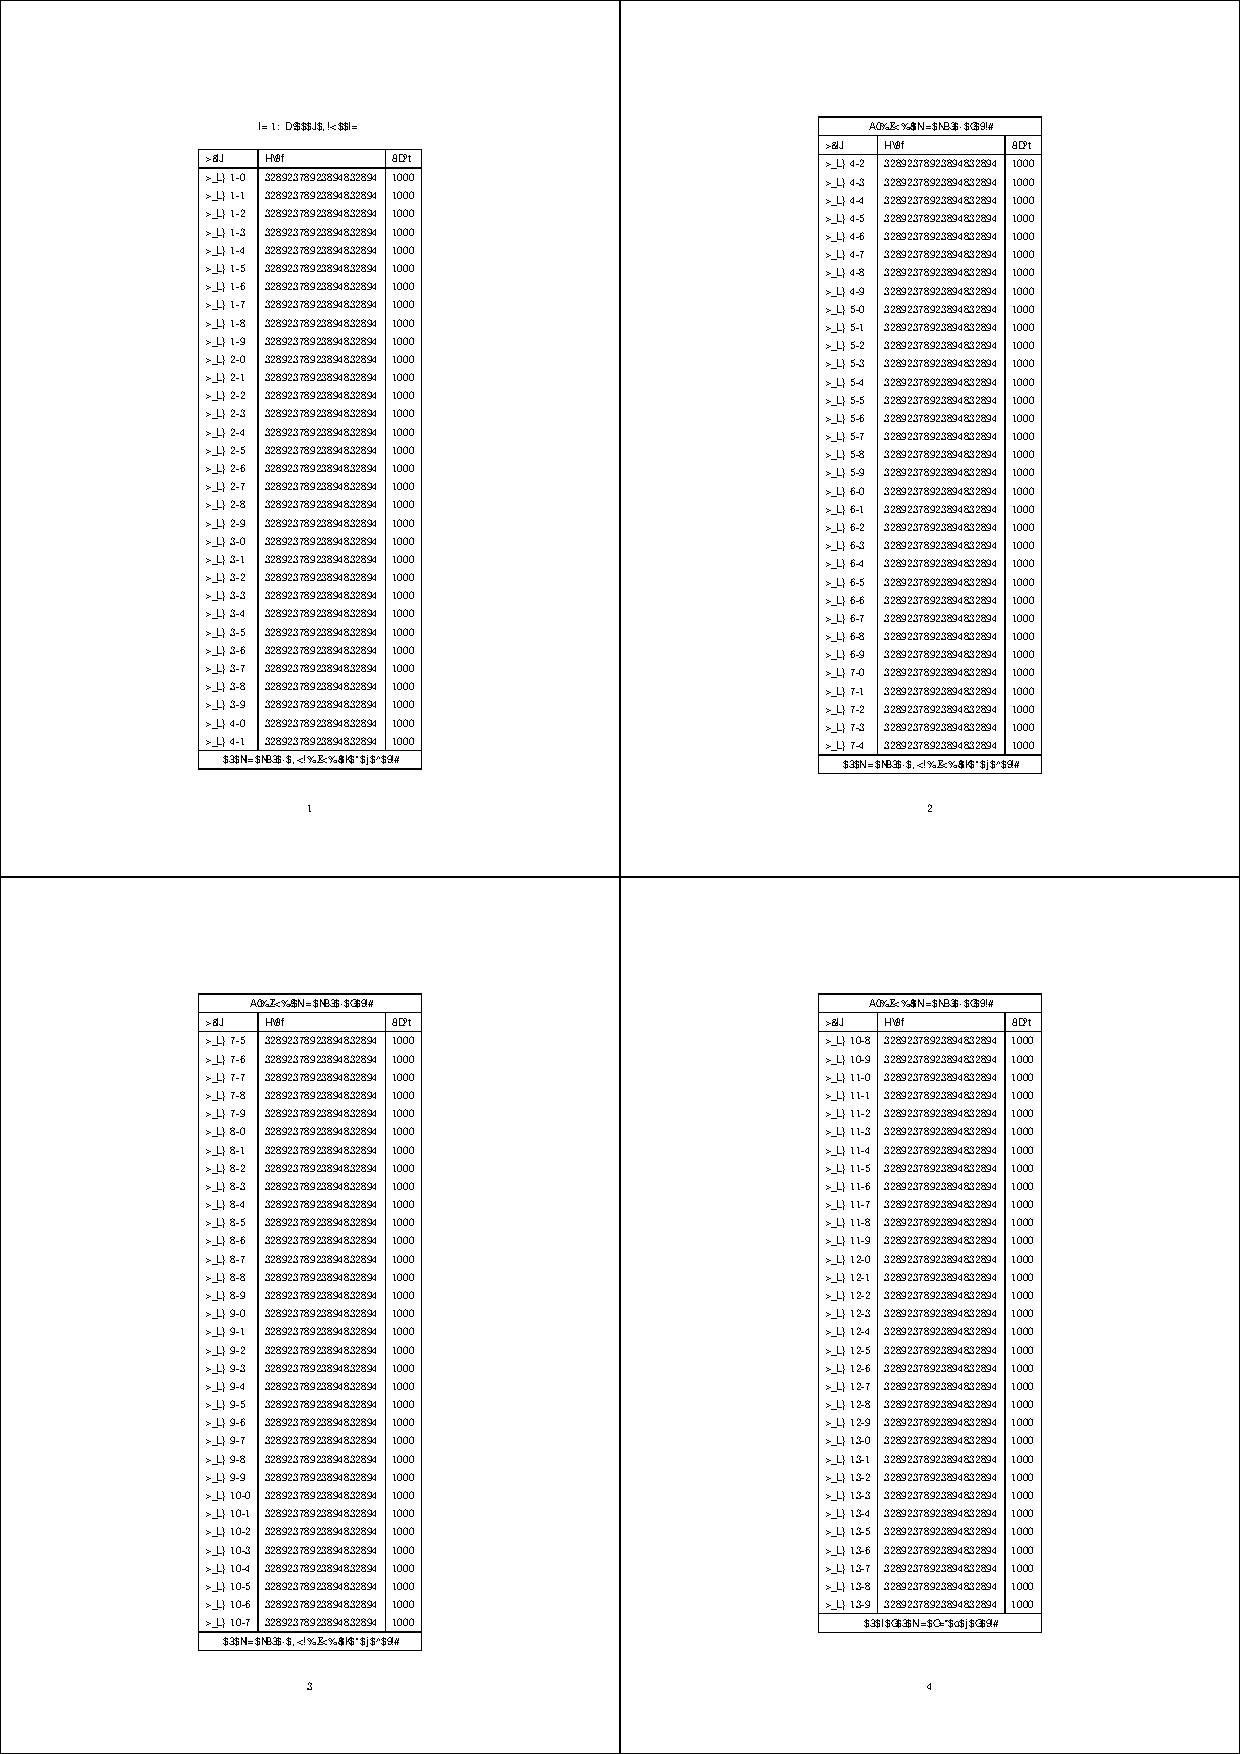
\includegraphics[width=\fullwidth]{images/longtable}%
   \IOlabel
   }%
   \caption{\Y{longtable}の使用例の出力結果}\label{fig:longtable}%
\end{figure}

\section{表の幅の指定\texorpdfstring{\zdash}{---}\Y{tabularx}}
\LaTeXe の \E{array}/\E{tabular} 環境では列の幅を直接指定できる
列指定子 `p\pa{width}' が用意されていますが、原稿を執筆している段階
ではその幅を決定できないことがしばしばあります。自動的にその幅を求め
てくれるような環境があれば便利です。そこで \ppl{David Carlisle}の作成
した \Y{tabularx} パッケージを用いることで \E{tabularx} 環境が使えます。
\begin{Syntax}
\C{begin}\verb|{tabularx}|\pa{幅}\pa{列指定子}\\
\va{表を構成する要素}\\
\C{end}\verb|{tabularx}| 
\end{Syntax}
具体例を以下に示します。
\begin{inputex}
\documentclass[a4j,10pt,papersize]{jsarticle}
\usepackage{tabularx}
\makeatletter
\def\hoge{\@tempcnta=\z@ \@whilenum \@tempcnta<10\do{%
   ほげほげ\advance\@tempcnta\@ne}。}
\makeatother
\begin{document}
\hoge%
 \begin{center}
  \begin{tabularx}{\linewidth}{|X|X|X|}
   \hline
   \hoge & \hoge & \hoge \\
   \hline
  \end{tabularx}
 \end{center}
\hoge%
\begin{center}
 \begin{tabularx}{\linewidth}{|r|l|X|l|X|}
  \hline
  商品   & 値段 & 説明  & 型番 & 補足事項 \\
  \hline
  鍋     &  500 & \hoge & 59A  & \hoge    \\
  \hline
  やかん &  300 & \hoge & 9JA  & \hoge    \\
  \hline
 \end{tabularx}
\end{center}
\hoge%
\end{document}
\end{inputex}
上記の入力例の出力例は\figref{fig:tabularx}となります。

\begin{figure}[htbp]
 \begin{center}
\makeatletter
\def\hoge{\@tempcnta=\z@ \@whilenum \@tempcnta<10\do{%
   ほげほげ\advance\@tempcnta\@ne}。}%
\makeatother
  \begin{tabularx}{\linewidth}{|X|X|X|}
   \hline
   \hoge & \hoge & \hoge \\
   \hline
  \end{tabularx}\par\vskip1em
 \begin{tabularx}{\linewidth}{|r|l|X|l|X|}
  \hline
  商品   & 値段 & 説明  & 型番 & 補足事項 \\
  \hline
  鍋     &  500 & \hoge & 59A  & \hoge    \\
  \hline
  やかん &  300 & \hoge & 9JA  & \hoge    \\
  \hline
 \end{tabularx}
\caption{\Y{tabularx}使用例の出力結果\label{fig:tabularx}}
\end{center}
\end{figure}
%
\E{tabularx} 環境において列指定子 `X' が新たに使えるようになっています。
\E{tabularx} 環境は組むべき表の幅を知る必要があります。`X' が複数の場合は
それぞれの列の幅は均等な長さになります。

\section{表における行の連結\texorpdfstring{\zdash}{---}\Y{multirow}}

\E{array}/\E{tabular} 環境で表などを作成していると、列の連結を
行なうことがしばしばあります。
\begin{InOut}
\begin{tabular}{lll}
\multicolumn{2}{c}{中央揃え} & ほげ\\
 ほげ & ほげ & ほげ\\
\end{tabular}
\end{InOut}
しかし、行の連結となると結構面倒です。そこで \ppl{Jerry Jeichter}と
\ppl{Piet Van Oostrum}による \Y{multirow} パッケージを使えば良いでしょ
う。
\begin{Syntax}
\C{multirow}\pa{行数}\pa{幅}\pa{要素}\\
\C{multirow}\pa{行数}\string*\pa{要素} 
\end{Syntax}
星を付けた場合は\va{要素}をLRモードで組んだときの幅で表を配置します。
まずは行を連結しない場合です。
\begin{InOut}
\usepackage{multirow}
\begin{tabular}{|l|l|l|}
\hline
\multicolumn{2}{|c|}{新商品}&旧商品\\
\hline
 なべ & やかん & たわし \\
\hline
\end{tabular} 
\end{InOut}
次は行を\va{要素}分の幅で連結した場合です。
\begin{InOut}
\begin{tabular}{|l|l|}
 \hline
 \multirow{2}*{新商品}
   & なべ \\
   & やかん \\
 \hline
 旧商品 & たわし \\
 \hline
\end{tabular} 
\end{InOut}
最後に全角 1 文字分の幅で行を四つ連結させた例です。ただし、
最後の行が 3 文字分あるため、幅の指定は効力がありません。
\begin{InOut}
\begin{tabular}{|c|l|}
 \hline
 \multirow{4}{1zw}{新商品}
   & なべ \\
   & やかん \\
   & コップ\\
   & 洗剤 \\
 \hline
 旧商品  & たわし \\
 \hline
\end{tabular}
\end{InOut}

%*** 他にもいっぱいあるよ (CTAN) [#t0f96e93]
%abstract, afterpage, bm, cite, color, comment, doublespace, epic, eepic, 
%fancybox, fancyhdr, graphicx, hyperref, indent, latexsym, layout, leftidx, 
%listings, pict2e, tex4ht, textcomp, theorem, url については初級編で
%すでに紹介しているので良いだろう。

%//*** csvtools  (CSV 形式のデータの読み込み)
%//手元にカンマ区切りとかタブ区切りの CSV データあって、それを LaTeX の
%//表などにして出力したいときは、自分でマクロを作ることも考えられますが、
%// による既存の csvtools パッケージを用いると良いでしょう。
%*** endfalot (図表は巻末に [#xc5df45a]

\section{巻末に図表を配置\texorpdfstring{\zdash}{---}\Y{endfloat}}

とある学会のスタイルで図表は巻末にまとめること、などという歴史的な
指定をされることが希にあります (昨今では図表を巻末にまとめなければ
ならないという技術的制約はほとんどなくなったと思いますが)。
これはには \ppl{James~D. McCauley}と \ppl{Jeff Goldberg}による 
\Y{endfloat} パッケージを使うことが考えられます。

パッケージオプションで図目次や表目次を表示させるか、どちらを先に
表示させるか等の設定が出来ます 
(\Optionlist{nofiglist,notablist,fighead,tabhead,nomarkers,tablesfirst})。

原稿で図表を記述している部分には \C{tableplace} や \C{figureplace} など
の定義が参照され、これが出力結果に反映されます。もし、本当に巻末にしかそ
れらを表示しないとなれば \Y{endfloat} パッケージを読み込んだ後に、
\begin{inputex}
\let\tableplace\empty
\let\figureplace\empty
\end{inputex}
などとすれば良いことになります。

\subsection{画像に文字を追加する\zdash\textsf{labelfig}}

\zindind{画像}{への文字の追加}%
再編集が難しい画像ファイル,例えば EPS ファイルの上に文字などのラベルを
追加したい場合があります.これには \Hito{Raymond S\'eroul} と
\Hito{Laurent Siebenmann} による \Y{labelfig} パッケージが使える
でしょう.
\begin{Syntax}
\C{SetLabels} \\
\va{画像の上に表示したいラベル}\\
\C{endSetLabels}\\
\C{ShowGrid} \pp{必要に応じて}\\
\C{strut}\C{AffixLabels}\va{配置する画像}
\end{Syntax}
\C{SetLabels} から \C{endSetLabels} の中で画像の上に表示したいラベルを
設定します.ラベルを追加するときに必要に応じて \C{ShowGrid} コマンドで
座標を表示します.\C{AffixLabels} の引数に配置すべき画像を指定します.
ラベルは次の書式に従って追加します.
\begin{Syntax}
\va{位置指定}\string(\va{0--1}\string*\va{0--1}\string) \va{ラベル} \verb|\\|
\end{Syntax}
座標指定は \verb|(0.5*0.3)| のように 0 から 1 の範囲で指定します.
\va{位置指定}には 垂直方向の揃えでは\C{T},\C{E},\C{B},
水平方向では \C{L}, \C{R} と無指定\pp{無指定で中央になる}の両方を
組み合わせて使うことが出来ます.

\C{ShowGrid} によってグリッドを表示するのは原稿執筆段階だけで,
印刷時には表示しないとなれば \Option{draft} オプションを活用します.
ただし,\sty{graphicx} パッケージによって読み込んでいる画像に関しては
\Option{draft} オプションが有効になっているときでも \Option{final} 
オプションを付けたときのように配置してもらいたいので,例えば
次のようにします.
\begin{InText}
% グリッドを表示させるのは draft の時だけにすれば良いことになる
%\documentclass[draft,a4j,11pt,papersize]{jsarticle}
% 印刷時には draft オプションを除けば良いことになる.
\documentclass[a4j,11pt,papersize]{jsarticle}
% graphicx パッケージには final を渡して,いつでも図が表示される
% ようにすると,labelfig の調整が容易になる.
\usepackage[final]{graphicx}
\usepackage{labelfig} 
\end{InText}

例えば次のような入力があれば \figref{fig:labelfig} のような出力に
なります.\C{GridLineWidth}コマンドで罫線の太さを指定できます.
\begin{InText}
\begin{figure}[htbp]
\begin{center}
 \GridLineWidth{.2pt}
 \SetLabels 
  \T\L(.8*.45) 鼻\\
  \T\L(.2*.9) 左の角\\
  \T\L(.7*.9) 右の角\\ 
  \T\L(.75*.3)  口\\ 
  \T\L(.65*.1) 髭\\ 
  \T\L(.3*.6) 左目\\ 
  \T\L(.7*.6)  右目\\ 
 \endSetLabels
 \ifdraft
   \ShowGrid
 \fi
 \strut\AffixLabels{
\includegraphics{images/gnu-head}}%
 \caption{labelfig の使い方\label{fig:you}}%
\end{center} 
\end{figure} 
\end{InText}

\begin{figure}[htbp]
\begin{minipage}{.49\linewidth}
 \GridLineWidth{.2pt}
  \SetLabels 
  \T\L(.8*.45) 鼻\\
  \T\L(.2*.9) 左の角\\
  \T\L(.7*.9) 右の角\\ 
  \T\L(.75*.3)  口\\ 
  \T\L(.65*.1) 髭\\ 
  \T\L(.3*.6) 左目\\ 
  \T\L(.7*.6)  右目\\ 
  \endSetLabels
  \ShowGrid
  \strut\AffixLabels{%
    
\includegraphics[clip,width=\linewidth]{images/gnu-head}}%
\end{minipage}
\hfil
\begin{minipage}{.49\linewidth}
  \SetLabels 
  \T\L(.8*.45) 鼻\\
  \T\L(.2*.9) 左の角\\
  \T\L(.7*.9) 右の角\\ 
  \T\L(.75*.3)  口\\ 
  \T\L(.65*.1) 髭\\ 
  \T\L(.3*.6) 左目\\ 
  \T\L(.7*.6)  右目\\ 
  \endSetLabels
  \strut\AffixLabels{%
    
\includegraphics[clip,width=\linewidth]{images/gnu-head}}% 
\end{minipage}
 \caption{\sty{labelfig} の使い方\label{fig:labelfig}}%
\end{figure}


%\section{画像にラベルを追加\texorpdfstring{\zdash}{---}\Y{labelfig}}
%再編集が難しい画像ファイル、例えば EPS ファイルの上に文字などのラベルを
%追加したい場合があります。これには \ppl{Raymond S\'eroul} と
%\ppl{Laurent Siebenmann} による \Y{labelfig} パッケージが使える
%でしょう。
%\begin{Syntax}
%\C{SetLabels} \\
%\va{画像の上に表示したいラベル}\\
%\C{endSetLabels}\\
%\C{ShowGrid} \pp{必要に応じて}\\
%\C{strut}\C{AffixLabels}\va{配置する画像}
%\end{Syntax}
%\C{SetLabels} から \C{endSetLabels} の中で画像の上に表示したいラベルを
%設定します。ラベルを追加するときに必要に応じて \C{ShowGrid} コマンドで
%座標を表示します。\C{AffixLabels} の引数に配置すべき画像を指定します。
%ラベルは次の書式に従って追加します。
%\begin{Syntax}
%\va{位置指定}\string(\va{0--1}\string*\va{0--1}\string) \va{ラベル} \verb|\\|
%\end{Syntax}
%座標指定は \verb|(0.5*0.3)| のように 0 から 1 の範囲で指定します。
%\va{位置指定}には 垂直方向の揃えでは\C{T}、\C{E}、\C{B}、
%水平方向では \C{L}, \C{R} と無指定\pp{無指定で中央になる}の両方を
%組み合わせて使うことが出来ます。
%
%\C{ShowGrid} によってグリッドを表示するのは原稿執筆段階だけで、
%印刷時には表示しないとなれば \Option{draft} オプションを活用します。
%ただし、\Y{graphicx} パッケージによって読み込んでいる画像に関しては
%\Option{draft} オプションが有効になっているときでも \Option{final} 
%オプションを付けたときのように配置してもらいたいので、例えば
%次のようにします。
%\begin{inputex}
%% グリッドを表示させるのは draft の時だけにすれば良いことになる
%%\documentclass[draft,a4j,11pt,papersize]{jsarticle}
%% 印刷時には draft オプションを除けば良いことになる。
%\documentclass[a4j,11pt,papersize]{jsarticle}
%% graphicx パッケージには final を渡して、いつでも図が表示される
%% ようにすると、labelfig の調整が容易になる。
%\usepackage[final]{graphicx}
%\usepackage{labelfig} 
%\end{inputex}
%
%例えば次のような入力があれば \figref{fig:labelfig} のような出力に
%なります。
%\begin{inputex}
%\begin{figure}[htbp]
%\begin{center}
% \SetLabels 
% \T\L(.2*.9) 揚力 $L$\\
% \T\L(.41*.95) 空気力 $R$\\
% \T\L(.47*.67) 抗力 $D$\\
% \T\L(.0*.53) 迎角 $\theta$\\
% \T\L(.03*.67) 翼弦線 $T$\\
% \T\L(.03*.37) 滑空方向 $N$\\
% \T\L(.4*.07) 重力 $G$\\
% \endSetLabels
% \ifdraft
%   \ShowGrid
% \fi
% \strut\AffixLabels{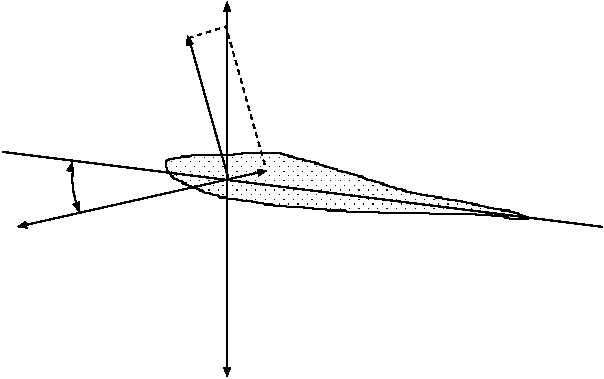
\includegraphics{samples/labelfig/youryoku}}%
% \caption{揚力の調整\label{fig:you}}%
%\end{center} 
%\end{figure} 
%\end{inputex}
%
%\begin{figure}[htbp]
% \begin{center}
%  \SetLabels 
%  \T\L(.2*.9) 揚力 $L$\\
%  \T\L(.41*.95) 空気力 $R$\\
%  \T\L(.47*.67) 抗力 $D$\\
%  \T\L(.0*.53) 迎角 $\theta$\\
%  \T\L(.03*.67) 翼弦線 $T$\\
%  \T\L(.03*.37) 滑空方向 $N$\\
%  \T\L(.4*.07) 重力 $G$\\
%  \endSetLabels
%  \ifdraft
%    \ShowGrid
%  \fi
%  \strut\AffixLabels{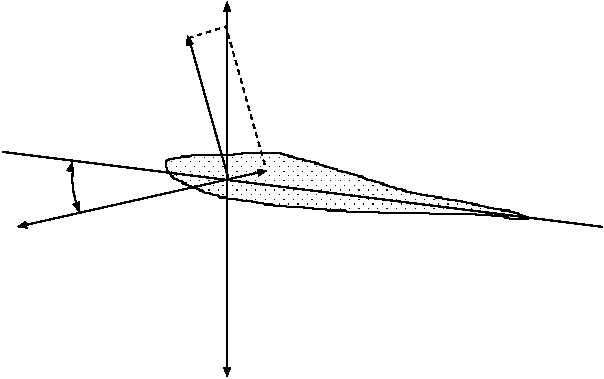
\includegraphics[clip,]{samples/labelfig/youryoku}}%
%  \caption{揚力の調整\label{fig:labelfig}}%
% \end{center} 
%\end{figure}



\section{図、表、そして写真\texorpdfstring{\zdash}{---}\Y{photo}}
%*** photo (図、表、写真というフロート [#y53aed71]
\LaTeXe 標準では 「図」のための \E{figure} 環境、「表」のための
\E{table} 環境が用意されていますが、ときどき「写真」のための \E{photo}
環境が欲しくなります。この場合、自分でマクロを作ることも考えられますが 
(中級編で紹介します)、\ppl{Volker Kuhlmann}による \Y{photo} パッケージ
を使うことが考えられます (高機能です)。

%パッケージオプションとしては以下のようなものがあります。
%:shortlop| \parskip が 0 ではないときにあいだが空かないようにきちんと
%「写真目次」を出力するためのもの。
%//:<見出し位置>| 標準では「写真」の見出しは写真の下端に出力されますが、
%//次のいずれかのパッケージオプションを渡すことで変更することが出来ます。

\E{figure}/\E{table} 環境と同様に \E{photo} 環境が用意されています。
星を付けると段を打ち抜きます。
\begin{Syntax}
\verb|\begin{photo*}|\\
\va{写真要素}\\
\verb|\end{photo*}|
\end{Syntax}

写真目次を出力するには \C{listofphotos} 命令を用います。
\begin{Syntax}
\C{listofphotos} % 写真目次の表示 
\end{Syntax}

浮動体の配置順序を指定するために \C{defaultphotoplacement} を適当に
`htbp' と定義しておきます。
\begin{Syntax}
\C{defaultphotoplacement}\pa{指定子}
\end{Syntax}
さらに \C{photoname} と \C{listphotoname} も
日本語で定義した方が良いでしょう。
\begin{inputex}
\def\photoname{写真}
\def\listphotoname{写真一覧} 
\end{inputex}


\E{photo} 環境以外にも \C{putphoto} 命令も使えます。
\begin{Syntax}
 \C{putphoto}\opa{位置}\pa{ラベル}\pa{小見出し}\pa{写真}%
 \opa{目次用見出し}\pa{見出し} 
\end{Syntax}
\va{小見出し} は内容がからで構いません (好みに応じて付け加えてください)。
\va{位置}には次の三つのグループから一つずつ選択できます。
\begin{description}
 \item[水平方向の揃え ] l (左側), r (右側), i (内側), o (外側)
 \item[垂直方向の揃え ] t (上部), c (中央), b (下部)
 \item[小見出しの位置 ] u (下側), s (左側)
\end{description}

\C{putphoto} 命令と同様に \E{Photo} 環境も用意されています。
\begin{Syntax}
 \verb|\begin{Photo*}|%
   \opa{位置}\pa{ラベル}\pa{小見出し}\opa{目次用見出し}\pa{見出し}\\
   \va{写真となる LR モード要素}\\
 \verb|\end{Photo*}|
\end{Syntax}

また「写真」を参照するには \C{phref}, \C{Phref} が使えます。
\begin{Syntax}
 \C{phref}\pa{ラベル}\\
 \C{Phref}\pa{ラベル} \pp{欧文で文の先頭に来た場合等に使える}
\end{Syntax}

ですから、これらをまとめると次のような使い方が出来ます。
出力例は\figref{fig:photo}となります。
\begin{inputex}
\documentclass[a4j,11pt,papersize,draft]{jsarticle}
\usepackage[shortlop,under]{photo}
\def\photoname{写真}
\def\listphotoname{写真一覧}
\oecaptionsep  0pt
\parskip   = 1zw
\newcommand\myphoto{\fbox{ここに写真がはいるはず\rule{30zw}{0pt}}}
\begin{document}
\parindent = 0zw
%
\listofphotos\clearpage
%
\begin{photo}[htbp]
 \begin{center}
  \myphoto% 写真の要素
  \caption{写真の見出し\label{ph:hoge}}
 \end{center}
\end{photo}
%
\putphoto{ph:foo}{}{\myphoto}[これはちょっとした例]{これはちょっとした例なんだ けど、
見出しがながーくなると自動的にあっちにふらふら}
\par
\phref{ph:hoge}とか \Phref{ph:foo} などなど。
\par
\putphoto[icu]{ph:piyo}{}{\myphoto}{位置を指定する}
\par
\begin{Photo}{ph:bar}{}{これも例}
 \myphoto
\end{Photo}
\renewcommand\myphoto{\fbox{ここに写真がはいる\rule{0pt}{9zw}}}
\par\noindent\putphoto[l]{ph:lhoge}{}{\myphoto}{位置を指定する}
\par\noindent\putphoto[r]{ph:rhoge}{}{\myphoto}{位置を指定する}
\end{document}
\end{inputex}
%
\begin{figure}[htbp]
   \IOmargin
   \makebox[0pt][l]{%
      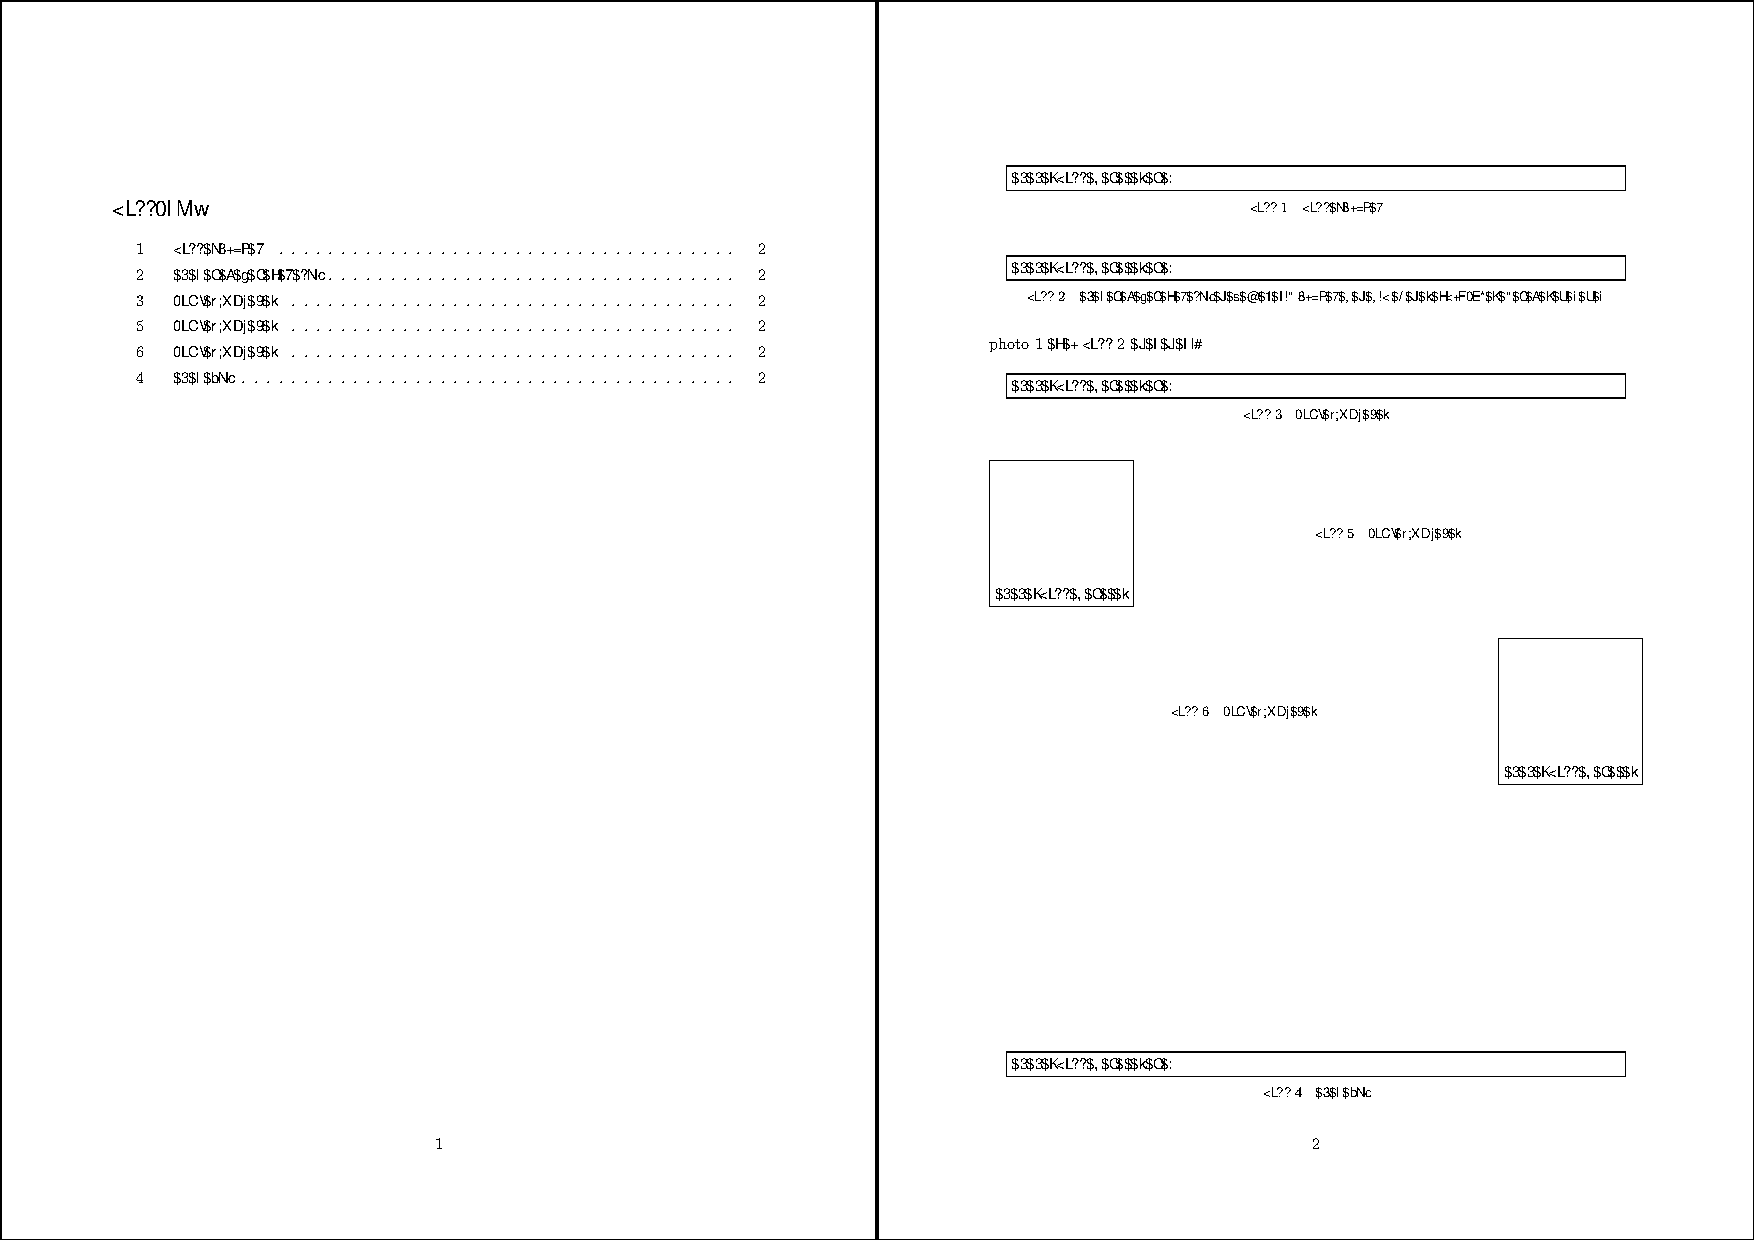
\includegraphics[height=\fullwidth,angle=-90]{images/photo}%
   \IOlabel
   }%
   \caption{\Y{photo}の使用例の出力結果}\label{fig:photo}%
\end{figure}


\clearpage
\null\vfill
\begin{flushright}
 
\includegraphics[scale=.4]{images/gnu-head}
\end{flushright}



